\chapter{Theoretische Grundlagen}
\label{cha:theogrund}

\section{Datenbank Entwurf / ERM}
\label{sec:erm}

Unter dem Datenbank Entwurf ist der Prozess zur Erstellung eines Schemas zu verstehen, welches die spätere Datenbank abbilden wird.
Hierunter fallen unter anderem die Analyse der Anforderungen, aber auch die grafische Darstellung der Tabellen, in denen die Daten gespeichert werden.
Der Entwurf der Datenbank im Voraus ist essentiell, da im späteren Prozess nderungen der Datenbankstruktur nicht nur die Datenbank selbst, sondern auch alle mit ihr verbundenen Applikationen betreffen wrden.
Um die Beziehungen korrekt darstellen zu können, wird das Entity-Relationship-Modell\footnote{vgl. Peter Pin-Shan Chen(1976): The Entity-Relationship Model--Toward a Unified View of Data. In: ACM Transactions on Database Systems, Vol 1, No 1, S.10} verwendet.
Durch diese Modell lassen sich sogenannte ER-Diagramme zeichnen, z.B. nach der Chen Notation\footnote{vgl. Peter Pin-Shan Chen(1976): The Entity-Relationship Model--Toward a Unified View of Data. In: ACM Transactions on Database Systems, Vol 1, No 1, S.19}.
Ein ER-Diagramm nach Chen stellt die Entittstypen (Klassen), Attribute, sowie Beziehungen (Relationen/Kardinalitäten) dar.
Im folgenden Beispiel soll ein ER-Diagramm nach der Chen-Notation kurz erläutertwerden.

\begin{figure}[H]
\begin{center}
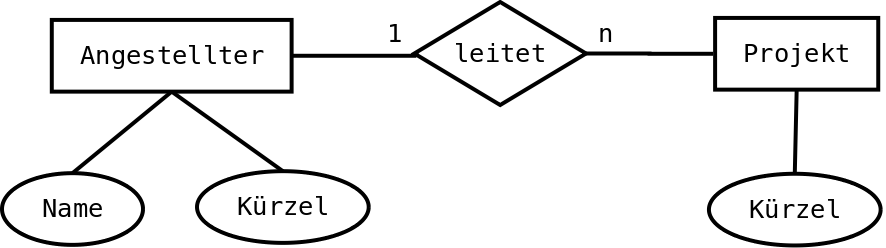
\includegraphics[scale=0.4]{img_chen_001.png}
\caption{Chen Notation 1:N}
\label{chenpic1}
\end{center}
\end{figure}
\footnotetext{In Anlehnung an Chen}


Das Diagramm beschreibt folgenden Sachverhalt:

\begin{itemize}
\item Ein Angestellter leitet mehrere Projekte.
\item Ein Projekt wird von einem Angestellten geleitet.
\end{itemize}

\begin{figure}[H]
\begin{center}
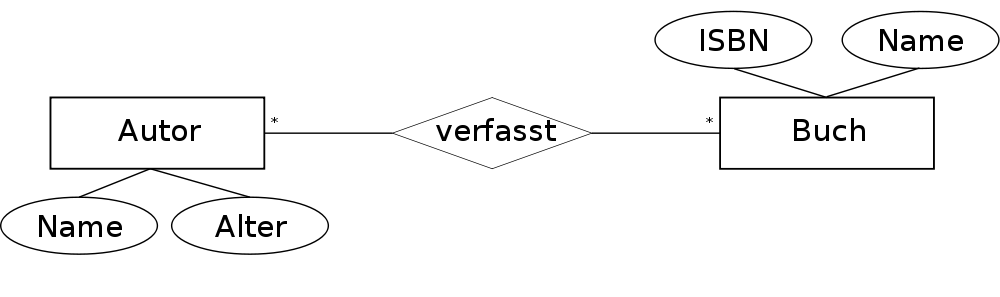
\includegraphics[scale=0.4]{img_chen_002.png}
\caption{Chen Notation N:M}
\label{chenpic2}
\end{center}
\end{figure}
\footnotetext{In Anlehnung an In Anlehnung an Quelle \cite{10}}

\begin{itemize}
\item Ein Autor verfasst mehrere Bücher.
\item Ein Buch wird von mehrere Autoren verfasst.
\end{itemize}



\section{Kardinalitäten}

Kardinalitäten beschreiben den Grad einer Verbindung zwischen zwei Objekten\footnote{vgl. Heinz Burnus(2007): Datenbankentwicklung in IT-Berufen, 1. Auflage, S.20}.
In Abbildung \ref{chenpic1} ist eine 1:n Kardinalitt gegeben.
Diese sagt aus, dass ein Objekt der Relation 1, mehrere Objekte der Relation 2 zugeordnet werden, einem Objekt der Relation 2 jedoch nur einem Objekt der Relation 1.

In der zweiten Abbildung \ref{chenpic2} ist eine n:m Kardinalitt zu sehen.
Diese sagt aus, dass ein Objekt der Relation 1, mehrere Objekte der Relation 2 angehören, einem Objekt der Relation 2 werden ebenfalls mehrere Objekten der Relation 1 zugewiesen.
Diese n:m Kardinalitäten müssen bei einem Datenbank Entwurf aufgelöst werden, da hier keine eindeutige Zuordnung möglich ist. Meistens lässt sich eine solche Kardinalitt wie in Abbildung \ref{chenpic2} durch das Hinzufügen einer zusätzliche Tabelle, welche beide Objekte verknüpft, lösen.
Ein Beispiel ist in Abbildung \ref{chenpic3} zu sehen.

\begin{figure}[H]
\begin{center}
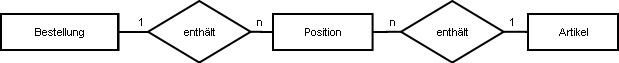
\includegraphics[scale=0.6]{chen_n_m_aufloesung.png}
\caption{Aufgelöste Chen N:M Notation}
\label{chenpic3}
\end{center}
\end{figure}

\section{Normalisierung - Optimierung von Datenbanken}
\label{secNormalisierung}
%\cite{codd1}
Wenn es bereits bestehende Datenbanken gibt, so muss geprüft werden, ob diese eine optimale Struktur aufweisen. Dies kann anhand der sogenannten Normalisierung durchgeführt werden.\footnote{vgl. E. F. Codd(1970): A Relational Model of Data for Large Shared Data Banks in Commun. ACM, Vol 13, Nr. 6, S. 381} Dadurch lässt die Datenbank sich weiter optimieren.\footnote{vgl. Prof. Dr. Paul. Alpar(2001): Vorlesung, Datenorganisation und Datenbanken,  http://www.tekinci.de/skripte/DBDM/DB-SS2001.pdf}
Bei der Normalisierung wird abgefragt, ob Tabellen gewisse Eigenschaften besitzen und passt diese wenn nötig an.
Hierzu stehen bis zu 5 Stufen der Normalformen zur Verfügung.
In der ersten Normalform wird untersucht, ob jedes Attribut atomare Werte besitzt, dass heißt es enthält nur einen Wert und ist frei von Wiederholungen.\footnote{vgl. Matthias Schubert(2007): Datenbanken, Theorie, Entwurf und Programmierung relationaler Datenbanken, 2. Auflage, S.293}


\begin{figure}[H]
\begin{center}
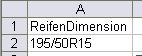
\includegraphics[scale=1]{img_chen_003.png}
\caption{Keine Normalform angewendet}
\label{chenpic4}
\end{center}
\end{figure}



In Abbildung \ref{chenpic4} ist eine Verletzung der Normalform 1. zu sehen. Um diese aufzuheben müssen wir die einzelnen Werte trennen wie in Abbildung \ref{chenpic5} zu sehen.

\begin{figure}[H]
\begin{center}
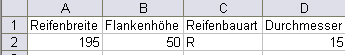
\includegraphics[scale=1]{img_chen_004.png}
\caption{1. Normalform}
\label{chenpic5}
\end{center}
\end{figure}

Wurde die Relation entsprechend angepasst, so ist Normalform 1 erreicht und es kann nun geprüft werden,
ob diese die Eigenschaften von Normalform 2 erfllt. Um eine Normalform zu erfüllen, müssen auch alle vorhergehende Normalformen erfllt sein, dass heißt erfllt eine Tabelle die Normalform 3, so erfllt sie auch die Normalform 1 und 2.
Die 5 wichtigsten Normalformen beschreiben sich durch folgende Attribute.\footnote{vgl. Heinz Burnus(2007): Datenbankentwicklung in IT-Berufen, 1. Auflage, S.292-308}

\begin{enumerate}
\item Normalform: Alle Attribute enthalten atomare Inhalte, und die Relation hat eine feste Breite
\item Normalform: Jedes Nichtschlüsselattribut ist vom kompletten schlüssel abhängig
\item Normalform: Jedes Nichtschlüsselattribut ist von keinem schlüsselkandidaten transitiv abhängig, dass heißt kein Attribut ist ber ein anderes vom Hauptschlüssel abhängig
\item Normalform: Es darf in einer Relation nicht mehrere, voneinander unabhängige, 1:n-Beziehungen zu einem schlüsselwert geben
\item Normalform: Eine weitere Aufspaltung ohne Informationsverlust ist nicht mehr möglich
\end{enumerate}



\section{DBMS}
\label{sec:dbms}


Ein Datenbankmanagementsystem organisiert die Speicherung der Daten einer Datenbank und legt die Anordnung der Daten fest.
Das DBMS legt auch die Art der Beziehung fest, in der die Daten der Datenbank stehen (relational, objektorientiert).
Zur Kommunikation mit diesem wird eine Sprache benötigt. Meist wird hier die deskriptive Sprache SQL verwendet.\footnote{vgl. E. F. Codd(1970): A Relational Model of Data for Large Shared Data Banks in Commun. ACM, Vol 13, Nr. 6, S. 382}


Es gibt verschiedene Arten von DBMS:

\begin{itemize}
\item Hierarchisch
\item Relational
\item Objektorientiert
\end{itemize}

%BuchURL http://www.amazon.com/gp/product/354043187X
Ein hierarchisches DBMS\footnote{vgl. Bernd-Jrgen Falkowski(2002): Business Computing: Grundlagen und Standardsoftware, 1. Auflage, S.235} dient vor allem der schnellen Suche in großen Datenbanken.
Der Nachteil liegt darin, dass nur eine sequentielle Abarbeitung möglich ist und somit die Art der Abfragen mehr oder weniger schon im Voraus bestimmt sein muss.
Im Gegensatz hierzu stehen die relationalen Datenbanken, welche heutzutage den höchsten Verbreitungsrad besitzen.
Diese bieten eine flexible Auswertung der Daten durch die deklarative Abfragesprache SQL.
Es muss lediglich die Verknüpfung zwischen den Tabellen durch sogenannte JOINs hergestellt werden, somit werden Primär- und Fremdschlüssel miteinander verknüpft.
Hinzu kommen die objektorientierten Datenbanken. Diese bieten die Möglichkeit Objekte aller Art zu speichern.
Problematisch hierbei sind jedoch die Formulierung von geeigneten Abfragen, weswegen diese in der Praxis eher selten und meist im Bereich von Multimedialenanwendungen anzutreffen sind.%\footnote{NOTIZ ODBMS evtl}

Wird versucht verschiedene relationale DBMS in der Praxis zu vergleichen, so ist eine große Anzahl an verschiedenen Systemen zu finden.
Eine kleine Auflistung soll einige Bekannte vorstellen.

\begin{itemize}
\item Microsoft Jet Engine (Access)
\item MS-SQL Server
\item Oracle
\item MySQL
\item PostgreSQL
\end{itemize}

Die Microsoft Jet Engine ist ein dateibasierendes DBMS, welches dem Benutzer eine einfache Möglichkeit bietet Daten in einer Datenbank zu speichern und passende Oberflchen (Frontends) in der Datenbank zu integrieren.
Wie alle anderen dateibasierenden DBMS bietet es die selben Vor- und Nachteile.
Bei diesem System steht meist die einfache Konfigurierbarkeit im Vordergrund. Die Datenbanken sind meist für einen Einzeluser-Betrieb ausgelegt und spielen hier auch ihre Stärken aus.
Wird eine dateibasierende Datenbank von mehreren Usern benutzt so zeigen sich die Nachteile eine solchen Datenbank.
Dadurch, dass Access für jeden Nutzer bei einer Abfrage die komplette Datenbank durchsucht entsteht eine hohe Auslastung der Festplatte, sowie des Netzwerks. Folglicherweise nimmt Geschwindigkeit bei mehreren Anwendern exponentiell ab, da sich alle Benutzer die Bandbreite der Festplatte sowie des Netzwerkes teilen.
Auch beim Speichern müssen zusätzlich Datensätze gesperrt und organisiert werden, weil sonst die Daten inkonsistent werden können, wenn mehrere Personen gleichzeitig einen Datensatz schreiben.
MS-SQL ist ebenfalls ein relationales Datenbankmanagementsystem und in den verschiedenen Serverbetriebssystemen von Microsoft enthalten.Für Entwickler ohne Lizenz wird eine eingeschrnkte Express Version zur Verfügung gestellt. MS-SQL ist im Gegensatz zu Access kein dateibasierendes DBMS, sondern ein DBMS welches zentral auf einem Server läuft.
Hierdurch werden die Nachteile des dateibasierenden zu den Vorteilen des serverbasierenden Systems.
Da der Server selbst die Abfragen verwaltet und zusätzlich Abfragen im Arbeitsspeicher ablegt, sowie dem Benutzer nur die Daten sendet, die er auch angefordert hat und nicht die komplette Datei, werden Zugriffszeiten und Netzwerk/Festplattenlast optimiert.

MySQL ist der Open Source Pendant zu MS-SQL, welcher im Internet eine sehr hohen Verbreitungsgrad aufweist.
So wird dieses von Seiten wie Wikipedia\footnote{vgl. Mysql, http://www.mysql.com/why-mysql/scaleout/wikipedia.html} oder
Youtube\footnote{vgl. University of Maryland: How YouTube scales MySQL for its large databases, http://ebiquity.umbc.edu/blogger/2007/12/28/how-youtube-scales-mysql-for-its-large-databases/} verwendet.
Im Gegensatz zu MS-SQL erlaubt das Lizenzmodell, dass die Datenbank für Privatanwender kostenlos ist und die Lizenzgebhren für Unternehmen einen Bruchteil der Kosten ausmachen, die für ein Microsoft System bezahlt werden mssten.\footnote{Vgl http://www.mindfactory.de/product\_info.php/pid/geizhals/info/p155132}

Eine weitere Datenbank stellt PostgreSQL dar, welches unter der BSD-Lizenz zur Verfügung gestellt wird und somit auch für kommerzielle Projekte ohne Kosten nutzbar ist\footnote{vgl. PostgreSQL: BSD-Lizenz, http://www.postgresql.org/about/licence}.


\section{Webserver}
\label{sec:websrv}

Ein Webserver dient zum Bereitstellen von statischen, sowie dynamischen HTML Seiten.
Der Vorteil bei Webservern liegt darin, dass nur Informationen ausgetauscht werden, die der Nutzer auch angefordert hat.
Weiterhin bietet es den Vorteil diese zielgerichteten Informationen einer größeren Menge an Benutzern zur Verfügung zu stellen, ohne dass spezielle Vorkehrungen zur späteren Skalierung getroffen werden mssen.

Um dynamische Webseiten erzeugen zu können, bedarf es einer Skriptsprache.
Aktuell haben sich folgende Sprachen etabliert:\footnote{vgl. Tiobe Software(2009): TIOBE Programming Community Index for August 2009, http://www.tiobe.com/index.php/content/paperinfo/tpci/index.html}

\begin{itemize}
\item ASP
\item JSP
\item PHP
\end{itemize}

ASP ist eine Skriptsprache der Firma Microsoft und basiert grundlegend auf der Syntax von Visual Basic.
JSP dient dem selben Zweck, wurde jedoch von Sun entwickelt und besitzt die Syntax von Java.
PHP ist eine Skriptsprache, welche sich hauptsächlich an der C Syntax orientiert und speziell für das Erstellen von
dynamischen Webseiten erstellt wurde. Sie ist die am weitesten verbreitete Scriptsprache zum Erstellen von dynamischen Webseiten.

Da alle der aufgeführten Skriptsprachen weitgehend Webserver-/Platformunabhängig sind, kann man frei zwischen den meist benutzten Webserverprogrammen whlen, hierunter fallen unter anderem:


\begin{itemize}
\item Apache
\item IIS
\end{itemize}

Der Apache Webserver ist ein Opensource Webserver der Apache Foundation.
Er kann unter vielen verschiedenen Betriebssystemen eingesetzt werden und untersttzt durch seine Module, alle verbreiteten Scriptsprachen, sowie Datenbanken.

Der IIS von Microsoft läuft ausschließlich unter Windows, zudem ist es auch nur unter dem Serverbetriebsystem von Windows möglich mehr als 10 Verbindungen gleichzeitig aufzubauen.\footnote{vgl. Microsoft: IIS 7.0: Übersicht ber die verfügbaren Features in IIS 7.0, http://msdn.microsoft.com/de-de/library/cc753198\%28WS.10\%29.aspx}

\section{Schnittstellen}
\label{sec:schnittstellen}


Um eine Verbindung zwischen den einzelnen Komponenten herzustellen, wird eine passende API bentigt.
Idealerweise bringt jedes DBMS und jeder Webserver passende Treiber mit, obwohl dieser Fall nicht immer gegeben ist.

Zur Zeit haben sich verschiedene Varianten etabliert:

\begin{itemize}
\item Native Treiber
\item ODBC (Open Database Connectivity)
\item JDBC (Java Database Connectivity)
\item ADO (ActiveX Data Objects)
\end{itemize}

Jedes etabliertes DBMS bietet für Entwickler eine native Schnittstelle zum Ansprechen der Datenbank an.
Diese wird meist in verschiedenen Programmiersprachen angeboten, unter anderem C/C++, PHP usw. .
Die native Methode besitzt den Vorteil, dass sie das Nutzen aller Funktionen der Datenbank ermöglichen, wohingegen dafür keine einheitlichen Design Pattern existieren, was die Verwendungen von mehreren
verschiedenen DBMS erschwert.

Aufgrund dessen hat sich in der Vergangenheit unter Windows das sogenannte ODBC etabliert, welches es ermöglicht ohne Modifizierung des Quellcodes, allein mit der Anpassung des DSN das DBMS zu wechseln.
Somit braucht der Entwickler sich nicht mehr mit Syntaxabweichungen zu beschäftigen, da er die ODBC Schnittstelle ANSI SQL konform ansprechen kann.
Neben dem ODBC gibt es auch ein JDBC System exklusiv für Java. Zwar kann Java auch ODBC ber die JDBC Schnittstelle nutzen, aber laut Sun \footnote{Vgl. Sun: JDBC-ODBC Bridge Driver, http://java.sun.com/j2se/1.3/docs/guide/jdbc/getstart/bridge.doc.html} soll die nur im experimentellen Gebrauch stattfinden.
Da der Einsatz eines nativen JDBC Treibers verhindert, dass keine unerwünschten Zustände auftreten, die z.B. bei einer JDBC-ODBC Treiber Brücke auftreten können.

Zusätzlich gibt es noch ADO von Microsoft, welches auch als Schnittstelle für Webserver mit IIS bzw. ASP dient.
Diese hnelt in der Logik JDBC, da ebenfalls ein ODBC-Treiber angesteuert werden kann.ü
Der Verbindungsaufbau ist ähnlich einfach gestaltet und ermöglicht auch für Webanwendungen eine einfache Anbindung an die Datenbank.

\section{Softwareentwicklung}
\label{sec:softdev}

\section{UML}
\label{sec:uml}

Die Unified Modeling Language (UML) ist eine standardisiertegraphische Modelierungssprache im Bereich der Softwareentwicklung. Der Standard wird von der Object Management Group verwaltet und wurde auch von dieser geschaffen. UML enthält verschiedene Notationstechniken um visuelle Modelle von softwareintensiven System zu erzeugen. UML selbst ist auch von der ISO standardisiert und zählt heutzutage zu einer der bedeutesten Modelierungssprachen bei der Softwareentwicklung. Durch die Sprache wird nicht nur eine grafische Notation festgehalten sondern ebenfalls die Begriffe und die jeweiligen Beziehungen zwischen diesen. Somit bilden die Diagramme nur eine Teil dessen ab, was unter der UML zu verstehen ist.
Die UML ist seit 1997 in Entwicklung und es gibt bisher mehrere Versionen von dieser.
Die verwendeten Modelle lassen sich in verschiedene Kategorien unterteilen, die wiefolgt lauten:\\
-Struktur-Diagramme\\
-Verhaltens-Diagramme\\
\\
In diese Kategorien lassen sich wiederum die in UML verwendeten Diagramme einordnen:\\
-Struktur-Diagramme\\
    * Klassendiagramm\\
    * Kompositionsstrukturdiagramm\\
    * Komponentendiagramm\\
    * Verteilungsdiagramm\\
    * Objektdiagramm\\
    * Paketdiagramm\\
    * Profildiagramm\\
-Verhaltens-Diagramme\\
    * das Aktivitätsdiagramm\\
    * das Anwendungsfalldiagramm\\
    * das Interaktionsübersichtsdiagramm\\
    * das Kommunikationsdiagramm\\
    * das Sequenzdiagramm\\
    * das Zeitverlaufsdiagramm\\
    * das Zustandsdiagramm\\
\\
Im folgenden soll nun auf die wichtigsten Diagramme eingegangen werden, welche im Projekt selbst verwendet wurden.\\
Das erste Diagramm, welches verwendet wurde, ist das Andwendungsfalldiagramm (im
folgenden als Usecase Diagramm benannt).  Dieses dient dazu einen Überblick über die Funktionen des Systems, aber auch über die beteiligten Personen (Akteure) zu erhalten. Das Usecase-Diagramm stellt keine Beschreibung der Abläufe dar, sondern die Beziehung zwischen Akteur und den jeweiligen Funktionen, die in diesem Fall als Anwendungsfall bezeichnet werden. Akteure können im Diagramm Anwender, Administratoren, aber auch Systeme selbst darstellen, welche von extern auf das System zugreifen. Im Diagramm selbst werden diese als ‘Strichmännchen ‘ dargestellt und haben jeweils einen Namen. In einem Usecase-Diagramm muss immer mindestens ein Akteur vorhanden sein.
Anwendungsfälle hingegen werden als Ellipsen dargeEin stellt und enthalten eine Beschreibung. Um beide unterschiedliche Elemente in einer Gruppe zusammenzufassen wird ein Rahmen um alle beteiligten Elemente gebildet, welcher Systemkontext genannt wird und somit die Systemgrenze darstellt. Neben den normalen Assoziationen (z.B. Benutzer -> Drucken) besteht die Möglichkeit der Generalisierung. Das bedeutet, dass zwei spezifische Akteure oder Anwendungsfälle zu einem generellen zusammengefasst werden können.
Ein Beispiel eines Usecase-Diagramms ist in Abbildung X zu sehen.\\
\\
\begin{figure}[H]
\centering
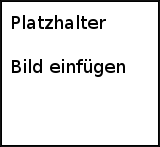
\includegraphics[width=0.3\textwidth]{000.PNG}
\caption{<BILDUSECASE>}
\label{fig:show_s1_s2_p1_n1}
\end{figure}
Ein weiteres wichtiges Diagramm stellt das Klassendiagramm dar. Es dient zur Beschreibung einzelner Klassen sowie deren Beziehungen untereinander. Klassen dienen zur Beschreibung der Objekte, welche von diesen instanziert werden. Im Klassendiagramm wird eine Klasse als Rechteck dargestellt und neben dem Klassenamen enthält diese ein Bereich für die Attribute, sowie für die Methoden. Um die Sichtbarkeit der Attribute und Methoden darzustellen werden verschiedene Symbole verwendet:\\

     + für public   unbeschränkter Zugriff\\
     \# für protected  , Zugriff nur von der Klasse sowie von Unterklassen (geerbte Klassen)\\
     \- für private  nur innerhlab der Klasse selbst sichtbar\\
     ~ für package  innerhalb des Pakets sichtbar\\
\\
Ähnlich wie bei dem Usecase-Diagramm bietet sich beim Klassendiagramm die Möglichkeit einer Generalisierung. Beispielsweise Sind die Klassen PKW und LKW Unterklassen von der Klasse Fahrzeuge. In Abbildung X ist ein Beispiel eines Klassendiagramms zu sehen.\\
\\
\begin{figure}[H]
\centering
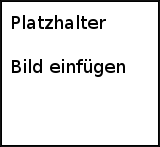
\includegraphics[width=0.3\textwidth]{000.PNG}
\caption{<BILDclass>}
\label{fig:show_s1_s2_p1_n1}
\end{figure}
Ebenfalls relevant für die Umsetzung des Projektes sind die Aktivitätsdiagramme. Sie dienen dazu Abläufe von Prozessen, aber auch von technischen Abläufen umzusetzten.
Beim Aktivitätsdiagramm befinden sich die Elemente in einem abgerundeten Rechteck, welche zusätzlich den Namen der Aktivität neben den Elementen enthält. Der Start bzw. Endpunkt bilden jeweils ein gefüllter Kreis, wobei der Endpunkt nur teilweise gefüllt ist. Aktivitäten werden in abgerundeten Rechtecken aufgelistet und miteinander in Flussrichtung verbunden. Entscheidungsfälle werden durch eine Raute symbolisiert. Je nach Entscheidungsfall, verläuft der Pfad bei ‘Ja’ weiter in Flussrichtung nach unten, oder bei einer Abweichung seitlich ab. Zusätzlich bietet sich die Möglichkeit Aktivitäten parallel ablaufen zu lassen. Dies kann durch Aktivitäten die zwischen 2 Balken angelegt werden, symbolisiert werden. Im foglenden ist in Abbildung X ein beispielhaftes Aktivitätsdiagramm zu sehen.\\
\\
\begin{figure}[H]
\centering
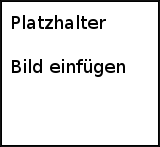
\includegraphics[width=0.3\textwidth]{000.PNG}
\caption{<BILDactivity>}
\label{fig:show_s1_s2_p1_n1}
\end{figure}
Für das bessere Verständnis der späteren Implementierung ist das Sequenzdiagramm ebenfalls von größerer Bedeutung. Es dient dazu ein Überblick über die Lebensdauer und Interaktion zwischen den einzelnen Klassen bzw. deren Objekte zu erhalten. Bei diesen wird nicht nur auf die bei den Klassendiagrammen gezeigte Beziehung sondern auch auf den Nachrichtenaustausch zwischen den Objekten eingegangen. Bei einem Nachrichtenaufruf mit Antwort bzw. mit einer daraus folgenden Aktion wird es notwendig zu unterschieden welche Art von Kommunikation stattfindet. Hierbei gibt es die synchrone, als auch asynchrone Kommunikation. Bei der zuerst genannten handelt es sich um ein Nachrichtenaustausch bei der das aufrufenden Element, beispielsweise ein Browser, dass Daten anfordert (eine Webseite). Hierbei sendet er die Anfrage für die jeweilige Seite ab und muss anschließend warten bis der Server ihm diese zurückgeliefert hat. Erst im Anschluss kann der die Webseite dem Nutzer darstellen.
Bei der asynchronene Kommunikation handelt es sich um ein Austausch, welcher es nicht erfordert, dass ein Teilnehmer auf die Bestätigung des anderen warten muss. Beispielsweise beim Versand einer Email. Hier muss der Sender weder warten bis der Empfänger online ist, noch muss er den Empfang der Email abwarten. Hier können Nachrichten gesendet werden, ohne dass für den Sender ein Ergebnis zur Laufzeit erwartet wird.
Eine Nachricht werden im Sequenzdiagramm durch Pfeile dargestellt. Synchrone Nachrichten werden mit gefüllten Pfeilspitzen, asynchrone Nachrichten mit offenen Pfeilspitzen gekennzeichnet. In der Nachfolgenden Abbildung ist ein beispielhaftes Sequenzdiagramm zu sehen.\\
\\
\begin{figure}[H]
\centering
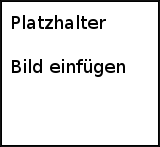
\includegraphics[width=0.3\textwidth]{000.PNG}
\caption{<BILDseq>}
\label{fig:show_s1_s2_p1_n1}
\end{figure}

\section{MAC - Media Access Control}
\label{sec:mac}

Bei der MAC-Adresse (Media-Access-Controll-Adresse) handelt es sich um eine Adresse eines Netzwerkadapters, die zur eindeutigen Identifizierung in einem Netzwerk dient. MAC-Adressen werden in einer Vielzahl von Netzwerk Protokollen verwendet. Unter anderem wird sie im Ethernet-Protokoll (IEEE 802.3)  aber auch vielen anderen Netzwerktechnologien genutzt die unter den IEEE 802 Gruppen zu finden sind.
Das MAC Protokoll steuert die Adressierung auf Hardwareebene, sowie die Zugriffsart.
Im IOS/OSI-Modell ist das MAC-Protokoll auf Schicht 2, der Sicherungschicht, angesiedelt.
Somit hat das MAC-Protokoll zwei Aufgaben, zum einen die Adressierung eines Gerätes und zum anderen wie dieses Gerät auf das Medium zugrreift.\\
Zur eindeutigen Adressierung der Netzwerkadapter  dient die sogenannte MAC-Adresse. Hierbei handelt es sich um einen 48-bit Wert, der einzigartig auf der ganzen Welt ist. Die ersten 24-bit kennzeichnen den Hersteller des Netzwerkadapters, die anschließenden 24-bit sind beliebig vom Hersteller vergebbar. Einige bestimmte MAC-Adressen können jedoch nicht reserviert werden, hierbei handelt  es sich um Broadcast-Adressen und Multicast-Adressen.
Eine MAC-Adresse kann wiefolgt dargestellt werden:\\
\\
01-23-45-67-89-ab\\
oder\\
01:23:45:67:89:ab\\
\\
Anhand der Herstellerkennung lassen sich wiederum Rückschlüsse auf das Netzwerkgerät schließen. Die Hersteller, welche jeweils hinter der Herstellerkennung sich verbergen sind öffentlich bei der IEEE einsehbar, z.B. per Internet.\footnote{http://standards.ieee.org/develop/regauth/oui/public.html}\\
Das MAC-Protokoll regelt ebenfalls den Zugriff auf das Transportmedium. Hierbei wird in zwei verschiedene Zugriffsarten unterteilt. Zum einen den kontrollierten Zugriff und zum anderen der konkurrierende Zugriff.
Beim kontrollierten Zugriff wird darauf geachtet, dass keine Kollision auftritt. Das bedeutet, keiner der Netzwerkgeräte kommuniziert gleichzeitig über einen Kanal, sondern es ist immer nur ein Gerät aktiv.\\
Beim konkurrierenden Zugriff hingegen darf jedes Gerät auf das Medium zugreifen, jedoch gibt es in diesem Fall bestimmte Regeln, wenn eine Kollision auftritt. In diesen wird geregelt in welcher Art und Weise die Kollisionen behandelt werden. In der Praxis gibt es unter anderem das Protokoll CSMA/CD. Dieses stellt bei einer Kollision durch ein Störr-Signal sicher, dass alle beteiligten Geräte die Kollision ebenfalls erkennen und versendet das Paket nach einer Zeit wiederum erneut bis dieses ankommt oder die Anzahl der maximalen Versuche überschritten wurde. Die warte Zeit steigt exponentiell anhand der Versuche . Hierzu wird eine Zufallszahl aus dem Bereich 0 und (2\^i)-1 gewählt.

\section{VLAN - Virtual Local Area Network}
\label{sec:vlan}

\section{SNMP}
\label{sec:snmp}
Unter dem Simple Network Management Protocol ist ein Netzwerkprotokoll zu verstehen, welches einem erlaubt Netzwerkgeräte (z.B. Drucker, Router, Switchs, Router) per Netzwerk zu überwachen und zu steuern.\footnote{vgl. Essential SNMP, S. 1}
Diese Abfragen werden von einem zentralen Punkt aus durchgeführt, dem sogenannten SNMP-Manager, welcher die Daten von den SNMP-Agenten (Netzwerkelementen) abruft.\footnote{vgl. Essential SNMP, S. 3}\\
Bei SNMP handelt es sich um ein Protokoll, welches sich auf der Schicht 7, die Anwendungs-Ebene, des ISO/OSI-Schichtenmodells, ansiedeln lässt.
Entwickelt wurde das Protokoll von der IEFT und ist über diverse RFCs definiert.
Durch die hohe Modularität ist SNMP auch unabhängig von IP und funktioniert somit auch über IPX oder AppleTalk. Dies ist mitunter auch ein Grund für die Weite Verbreitung von SNMP, welches mittlerweile als Standard gilt.\\
Die Funktionsweise von  SNMP spiegelt sich in der Verwendung der Agenten und Manager wieder.
Zunächst gibt es die sogenannten Agenten welche als Dienst auf dem jeweiligen Endgerät laufen und die Informationen zur Verfügung stellen. Diese werden dann auf einem Manager jeweils abgerufen per SNMP. Die Nachrichten werden entweder angefordert vom Manager oder aufgrund eines Ereignisses vom Agent an den Manager selbständig gesendet.\\
SNMP selbst definiert nicht welche Daten/Werte die Netzwerkkomponenten liefern, sondern gibt nur eine Baumstruktur vor, an die sogennante Management Information Base (MIB) angliedert.
Diese beschreibt die jeweils enthaltenen Informationen und sind teilweise ebenfalls über RFCs spezifiziert.\footnote{vgl. RFC 1213} Zusätzlich gibt es herstellerspezifische MIBs z.b. von Cisco , die in einem speziellen Punkt im Baum hinterlegt werden können. Diese MIBs werden unter dem  Object Identifier (OID) 1.3.6.1.4.1 (iso.org.dod.internet.private.enterprises) bei der IANA registriert.\\
Bei der Kommunikation untereinander werden verschiedene Paket-Typen verwendet.
Diese sind wiefolgt:\\
GET\\
GETNEXT\\
GETBULK\\
SET\\
RESPONSE\\
TRAP\\


Bei den GET Paketen handelt es sich um jeweils unterschiedliche Arten der Anforderung die vom Manager an den Agent gesendet werden.\\
Bei einem normalen GET-Paket wird ein einzelnes Attribut vom Agenten angefordert. Jedoch gibt es Abfragen, bei denen nicht im Voraus bekannt ist, wie viele Attribute abgefragt werden müssen. Beispielsweise der Status mehrerer Ports an einem Switch. Da dem SNMP-Manager jedoch keine Informationen vorliegen wie viele Ports der Switch hat, kann er nicht im Voraus die entsprechende Abfrage starten.\\
Um diese Problematik zu lösen gibt es den sogenannten GETNEXT-Befehl, der es ermöglicht den Wert sowie die OID eines daraufolgenden Elementes zu erhalten.\\

//<Beispiel>\\

Die Abfrage von x Ports erzuegt x+1 Abfragen (Bei einem 48+2 Port Switch somit 51 Abfragen) ist neffektiv , da der Manager nur eine Informationsmenge erhalten möchte aber dazu eine vielzalh an Anfragen durchführen muss. Daher wurde mit SNMP v2 der GETBULK Befehl eingeführt. Dieser ermöglicht es mehrere Werte mit einer Abfrage zu erhalten, die am Knoten im Baum hinterlegt sind.\\
Das SET-Paket dient zum setzten spezieller Werte, so kann zum Beispiel darüber der Status des Portsvon einem Switch  geändert werden, oder es könnte eine Firewall konfiguriert werden.
Auf diese bisher genannten Pakete antwortet der Agent mit einem RESPONSE Paket, welcher die benötigten Werte oder eine Fehlermeldung enthält.
Sofern beim SNMP-Agent z.B. gewisse Grenzwerte hinterlegt wurden kann dieser sich bei einer Überschreitung mittels eine Trap-Paketes beim Manager melden, ohne das dieser die Information explizit abgefragt hat.\\
Um möglichst wenig Netzwerklast zu erzeugen kommuniziert SNMP über das UDP Protokoll, da es eine Verbindunglose Kommunikation ermöglicht. Der Agent erhält die Anfragen auf Port 161, während der Manager auf Port 162 die Trap Meldungen empfängt.\\

\section{CDP - Cisco Discovery Protokoll}
\label{sec:cdp}

Das CDP von Cisco ist ein propäriteres Protokoll, welches dazu dient, Cisco-Geräten zu ermöglichen andere angeschlossene Geräte zu identifizieren und mit diesen Informationen auszutauschen. Es kann allerdings auch zum sogennanten “On-Demand-Routing” verwendet werden. Hierbei handelt es sich um eine cisco-spezifische Erweiterung von CDP, welche es ermöglicht ein simples Routing zu erstellen.
Die Cisco Geräte senden jeweils zur Multicast -Adresse “01-00-0c-cc-cc-cc”, welche auch von anderen Cisco-Protokollen (Z.B. VTP) verwendet wird. Dies geschiet in einem Intervall von 60 Sekunden auf allen relevanten Interfaces. Jedes der beiteiligten Cisco Geräte führt intern eine Tablle mit den Informationen über die Geräte, welche in der “Nachbarschaft” gefunden wurden. Hierunter fallen Dinge wie IP, Alias, Geräte-Typ und auch Informationen über die dort befindliche Software bzw. das Betriebsystem. Bei einem Cisco-Swicth wird zum Beispiel nicht nur die Beschreibung (IOS) sondern Modell, IOS-Version, Gegenstelle des Ports auf dem anderen Gerät, Link-Status (Geschwindigkeit, Duplex), aber auch VLAN und viele weitere Informationen. Diese können per internen Befehl oder per SNMP abgefragt werden. Bei jedem Empfang von CDP Daten, werden die internen Tabellen gepflegt und die Haltbarkeitszeit wieder zurückgesetzt, da Geräte die sich nicht mehr melden nach einer bestimmten Zeit (Standardmäßig nach 180 Sekunden) aus den Tabellen wiederum entfernt werden. Die Informationen welche übertragen werden sind einfach erweiterbar, da diese auf dem “Type-Length-Value” Format basieren. Das heißt in einer Nachricht wird zuerst der Typ des Attributs bestimmt (Z.b. String, Zahl, Datum) danach die (Zeichen-)Länge des Wertes und der Wert selbst.\\
Hersteller wie HP, distanzieren sich zunehmend von diesem properitären Protokoll und unterstützen das durch die IEEE spezifizierte offene Protokoll LLDP, welches Hersteller unabhängig ist und den selben Funktionsumfang beinhaltet.